\documentclass{article}
\usepackage[utf8]{inputenc}
\usepackage{breakurl} 
\usepackage [english]{babel}

\usepackage [autostyle, english = american]{csquotes}

\MakeOuterQuote{"}

\usepackage{hyperref}
\usepackage{natbib}
\usepackage{graphicx}
\usepackage[margin=1in]{geometry}


\title{Using Geolocated Tweets to Measure Future Orientation}
\author{Joel McGuire \thanks{Department of Economics, University of Oklahoma.\
E-mail~address:~\href{mailto:
joel.p.mcguire-1@ou.edu}{Joel.p.McGuire-1@ou.edu}} & Donald Li }
\date{May 2018}





\begin{document}

\maketitle



\begin{abstract}
\begin{singlespace}
We construct a measure of future orientation from geolocated tweets using sentiment analysis and find some evidence of its validity by regressing the index against several metrics that research suggests will be related to future orientation. Further research needs to conducted before reaching any conclusions about the viability of twitter to measure aggregate expectations. 
\end{singlespace}

\end{abstract}
\vfill{}


\pagebreak{}


\section{Introduction}
Future orientation is a dimension of intrapersonal and intercultural psychology with ties to health and economic metrics. Evidence suggests it has the capacity to predict growth and savings rates on a national level as well as economic and health behaviors on an individual scale.

\section{Literature Review}

\subsection{Future Orientation}


Time perspective is a fundamental psychological dimension humans use to frame experienced reality as belonging to the past, present, or future \citep{zimbardo2015putting}. Whether one is more oriented towards the future or present is deeply related to self regulation \citep{howlett2008role}. Research has been shown that the time orientation of people are related to health behaviors. People who are more future orientated are shown to be more likely to engage in health positive behaviors. Such as moderation of ones diet, use of mind altering substances, seat belt use, etc. While people who are more present orientated are shown to be more likely to engage in health negative behaviors such as excessive consumption of alcohol, drugs and risky sex.  \cite{henson2006associations},  \cite{daugherty2010taking}.\\ These effects persist even when demographic factors such as age, sex, and income are accounted for. 

Among other factors such as financial literacy and risk preference, future orientation affects personal savings rate. Future orientated person's are more likely to save both on an individual level \citep{jacobs2005influence}, and as a country \citep{hofstede1988confucius, hofstede1991cultures}. Read, cited by Hofstede, found that a country scoring higher on an index of long term orientation is positively related to the marginal propensity to save \cite{read1993politics}.


Time orientation has also been found to have an effect on savings even at a macro level. \cite{hofstede1988confucius}. Using the Chinese as a case study researchers found Asian cultural norms lean towards the avoidance of uncertainty. This leads to an increase in personal savings as to hedge against the future.  \citep{hofstede1988confucius}. 

\subsection{Twitter as a Social Science Tool}

The use of twitter for social science research has grown in recent years. Mitchel and colleagues used sentiment analysis to create a new index of happiness by city in the USA \citep{mitchell2013geography}. Most closely related in methodology is the the work done to predict HIV rates on a county level using an index of geolocated future oriented tweeted \citep{ireland2015future}. Twitter has also been used to predict instances of crime \citep{gerber2014predicting}, elections results \citep{tumasjan2011election}, and of course future movements of the stock market \citep{bollen2011twitter}. An economic way of considering future orientation is by considering that the parameter that controls how one discounts the future may be tuned by culture. If one is more likely to identify with a future self they are less likely to act inconsistently. Saving more is the most obvious representation of a continuity of self.   


\subsection{Time Perspective and the Internet}

Prior research has created a future orientation index from Google search terms of a countrywide level \citep{preis2012quantifying}. There is extremely limited research that establishes if an index of future orientation may be constructed from geolocated tweets for a more granular geographic region. We seek to find if such an index has any ability to predict factors related to future orientation on a state level, or metropolitan area.

In the vein of Chen's work on how language itself changes inter-temporal choice, finding that "languages that grammatically associate the future and the present foster future-oriented behavior" (2013), we hypothesize that areas with relatively future oriented tweets will have higher savings rates. Since such data is unavailable we will use interest in savings accounts as a proxy for savings rates. 

A shortcoming of previous metrics of future orientation are an inability to capture changes in culture, primarily by the assumption of cultural being relatively invariant \citep{tang2008framework}. Benefits to this method are that it opens an avenue to the possibility of creating a dynamic understanding of cultural change through language, and an ability to compare that relationship with macroeconomic indicators.

The missing piece in the literature is whether there are robust and consistent cultural differences between states or regions of the USA. If there are no such significant differences then goal of measuring those differences using twitter becomes a moot point. 

\section{Methodology}

\subsection{Data Source}
Tweets were collected from Twitter. 
Tweets were streamed using the Twitter API (N = 53,007,230) from February 2018 to April 2018. Once the number of tweets were filtered by geo-location, the number of tweets was reduced to 4,617,981. A higher recovery rates are possible but most methods to do so are either computationally or monetarily costlier. This would be done by referencing the users self identified location and using relatively straightforward NLP procedures to parse this string into latitude and longitude coordinates. Additionally, only tweets were used that were written in English. While this is necessary for the analysis it raises some question regarding the potential unrepresentative nature of scores for states with large Spanish speaking populations. Twitter as a whole is unrepresentative of the greater population, but if it gives a sample that is consistently biased for each state then it should still be useful for the intended analysis.  

The dictionary of future, present, and past oriented words was retrieved from the LIWC. 
GDP growth rate was retrieved from the Bureau of Economic Analysis. Most problematic is the current inability to match any macroeconomic indicator to this small window of twitter sentiment retrieved. The optimal metric of comparison would be personal savings rate by state but so far that information appears to be not easily attainable. Google search data was retrieved from google trends \footnote{https://trends.google.com/trends/}. ACT scores for 2017 were retrieved from www.act.org and SAT scores were downloaded from college board \footnote{https://research.collegeboard.org/programs/sat/data}  \footnote{http://www.act.org/content/act/en/research/condition-of-college-and-career-readiness-2017.html}.


\subsection{Analysis Strategy}
A simple approach to natural language processing was used to create our future orientation index for each state of the United States. Implementing the 2015 dictionary of the Linguistic Inquiry and Word Count (LIWC), an extensively validated tool for text analysis, was used to identify a set of future oriented words such as "gonna", "will", and "hope" \cite{pennebaker2015development}. These words that have been previously identified as relating to a longer time perspective were aggregated per state. The index was created by taking the difference of the the sum of all future oriented words in a state and the the sum of the past and present associated words found in tweets geolocated in a particular state. 

Even though we do naively regress the index of future orientation on the nearest data we have on GDP growth rate, we acknowledge there is little reason to suggest they would be related. We must wait for the data to catch up. 

We chose our geographical unit of analysis for the state due to the constraints on data available to validate our results on a more granular level.

To validate our index we use simple OLS to regress our index against GDP growth, average state math ACT and SAT scores, and the relative interest of each state over the same time period in savings. This was measured by proxy using the popularity of searches for "savings account" per state from google trends. Searches for "savings" were not used as a proxy for interest in savings behavior due to all related queries being reported as having to do with daylight savings, while for "savings account" the related queries normally have to do with banks. 

\subsection{Models}

\[ \scalebox{1.5}{ $O_s = \frac{\sum^p_1 I(w \epsilon D_1) + \sum^c_1 I(w \epsilon D_2 ) - \sum^f_1 I(w \epsilon D_3 ) }{n}  $} \]

$O_s$, the not-future orientation by state is determined by the sum of the sums of the score of how many words $w$ are in the $D_1$ the past oriented dictionary, $D_2$ the present oriented dictionary, and $D_3$ the future oriented dictionary. 
This difference was divided by $n$ which is the total number of words tweeted in a state during the period of analysis. 



\subsection{PROBLEMS}

\begin{enumerate}
    \item There is not any data for savings rate on the state level. Alternatives: Growth in investment related industry, financial services perhaps, what about change in personal consumption? Venture capital on the metropolitan level? 
    \item As previously noted, future orientation is naturally predicts future behavior. It is awkward and causally inert to compare present metrics of future orientation to present behavior. For the best results it is appropriate to collect tweets as a time series, and use it to predict changes in the USA personal savings rate. 
    \item Research indicating cultural differences between states with regards to intertemporality is a necessary prerequisite for validating any index that attempts to establish a connection between future orientation expressed in speech and behavioral differences between groups.
  
\end{enumerate}

\section{Results}
Refer to table 1 and Table 2 for the results of the OLS regression. The results of two out of our four regressions are positive, one is ambiguous, and the fourth is negative. The negative results is that we see no significance for the coefficient for our index of non future oriented tweets. Our index has a significantly positive relationship with GDP growth during the last year. Since growth is often spurred by consumption, it is unclear whether this reflects that our index is measuring what we intend it to measure. Lastly we have slightly significant coefficients for the index positively relating to an increase in search interest in "savings account" and the average ACT math score. 

\section{Conclusion}

Our index shows a relationship between future orientation on a state level and several metrics commonly tied to being more future orientated. Results are mixed as some regressions are not significant. Further research is required to provide more evidence as to the efficacy of twitter as a tool to extract future sentiment of an area. 

\pagebreak{}

\bibliographystyle{apalike}
\bibliography{PS11_McGuire.bib}

\pagebreak{}
\section{Appendix}

\begin{figure}[h!]
\centering
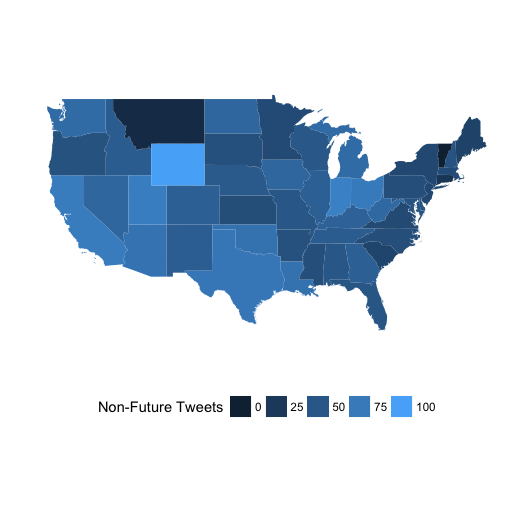
\includegraphics[width=10cm,height=10cm]{Non_future_tweets.png}
    \caption{US_future_sentiment}
\end{figure}



\begin{table}[!htbp] \centering 
  \caption{OLS} 
  \label{} 
\begin{tabular}{@{\extracolsep{5pt}}lcc} 
\\[-1.8ex]\hline 
\hline \\[-1.8ex] 
 & \multicolumn{2}{c}{\textit{Dependent variable:}} \\ 
\cline{2-3} 
\\[-1.8ex] & GDP Growth 2017 & State Math SAT \\ 
\\[-1.8ex] & (1) & (2)\\ 
\hline \\[-1.8ex] 
 Non Future Tweet Index & 3.629$^{***}$ & 28.965 \\ 
  & (1.211) & (44.683) \\ 
  & & \\ 
 Constant & $-$6.559$^{**}$ & 488.011$^{***}$ \\ 
  & (2.920) & (107.718) \\ 
  & & \\ 
\hline \\[-1.8ex] 
Observations & 49 & 49 \\ 
R$^{2}$ & 0.160 & 0.009 \\ 
Adjusted R$^{2}$ & 0.143 & $-$0.012 \\ 
Residual Std. Error (df = 47) & 1.307 & 48.200 \\ 
F Statistic (df = 1; 47) & 8.977$^{***}$ & 0.420 \\ 
\hline 
\hline \\[-1.8ex] 
\textit{Note:}  & \multicolumn{2}{r}{$^{*}$p$<$0.1; $^{**}$p$<$0.05; $^{***}$p$<$0.01} \\ 
\end{tabular} 
\end{table} 



\begin{table}[!htbp] \centering 
  \caption{} 
  \label{} 
\begin{tabular}{@{\extracolsep{5pt}}lcc} 
\\[-1.8ex]\hline 
\hline \\[-1.8ex] 
 & \multicolumn{2}{c}{\textit{Dependent variable:}} \\ 
\cline{2-3} 
\\[-1.8ex] & State ACT Math & State Searches for "Savings Accounts" \\ 
\\[-1.8ex] & (1) & (2)\\ 
\hline \\[-1.8ex] 
 Non Future Tweet Index & $-$3.622$^{**}$ & $-$20.913$^{**}$ \\ 
  & (1.789) & (9.349) \\ 
  & & \\ 
 Median Household Income &  & 0.001$^{***}$ \\ 
  &  & (0.0002) \\ 
  & & \\ 
 Constant & 29.964$^{***}$ & 76.203$^{***}$ \\ 
  & (4.313) & (25.303) \\ 
  & & \\ 
\hline \\[-1.8ex] 
Observations & 49 & 49 \\ 
R$^{2}$ & 0.080 & 0.282 \\ 
Adjusted R$^{2}$ & 0.061 & 0.251 \\ 
Residual Std. Error & 1.930 (df = 47) & 9.998 (df = 46) \\ 
F Statistic & 4.097$^{**}$ (df = 1; 47) & 9.048$^{***}$ (df = 2; 46) \\ 
\hline 
\hline \\[-1.8ex] 
\textit{Note:}  & \multicolumn{2}{r}{$^{*}$p$<$0.1; $^{**}$p$<$0.05; $^{***}$p$<$0.01} \\ 
\end{tabular} 
\end{table} 



\end{document}
